\documentclass[10pt, anonymous, conference]{IEEEtran}
\IEEEoverridecommandlockouts

% --- Symbols & Custom Marks ---
\usepackage{pifont}
\newcommand{\cmark}{\ding{51}}
\newcommand{\xmark}{\ding{55}}
\newcommand{\pmark}{\ding{109}} % partial coverage

% --- Core Packages ---
\usepackage{cite}
\usepackage{amsmath,amssymb,amsthm,amsfonts}
\usepackage[expansion=false]{microtype}
\usepackage{booktabs, multirow}
\usepackage{xcolor}
\usepackage{graphicx}
\usepackage{textcomp}

% --- Visualization & Plots ---
\usepackage{tikz}
\usepackage{pgfplots}
\pgfplotsset{compat=1.18}
\usepgfplotslibrary{statistics,groupplots}
\usetikzlibrary{arrows.meta,positioning,shapes.geometric,automata,fit,backgrounds,calc}

% --- Algorithms & Code ---
\usepackage{algorithm}
\usepackage{algpseudocode}
\usepackage{listings}

% --- Layout & Utility ---
\usepackage{mdframed}
\usepackage{enumitem}
\usepackage{hyperref}
\usepackage{cleveref}

% --- Theorem environments ---
\theoremstyle{definition}
\newtheorem{definition}{Definition}[section]
\newtheorem{example}{Example}[section]
\newtheorem{problem}{Problem Statement}[section]
\newtheorem{assumption}{Assumption}
\renewcommand{\theassumption}{A\arabic{assumption}}
\theoremstyle{plain}
\newtheorem{theorem}{Theorem}[section]
\newtheorem{proposition}{Proposition}[section]
\newtheorem{lemma}{Lemma}[section]
\newtheorem{corollary}{Corollary}[section]
\theoremstyle{remark}
\newtheorem{remark}{Remark}[section]

% --- Running-example box ---
\newmdenv[
  backgroundcolor=gray!7,
  linecolor=black!25, linewidth=0.5pt,
  topline=true, bottomline=true, leftline=true, rightline=true,
  innertopmargin=7pt, innerbottommargin=7pt,
  innerleftmargin=9pt, innerrightmargin=9pt,
  skipabove=9pt, skipbelow=9pt
]{runbox}

% --- Listing style (view-metamodel / rule snippets) ---
\lstset{frame=single, backgroundcolor=\color{gray!5},
        basicstyle=\ttfamily\scriptsize, breaklines=true,
        showstringspaces=false, numbers=none}

% --- Custom Commands ---
\newcommand{\finding}[1]{\smallskip\noindent\textbf{Finding:} \textit{#1}\smallskip}
\algnewcommand{\LineComment}[1]{\State \(\triangleright\) \textit{#1}}
\algnewcommand\algorithmicinput{\textbf{Input:}}
\algnewcommand\algorithmicoutput{\textbf{Output:}}
\algnewcommand\Input{\item[\algorithmicinput]}
\algnewcommand\Output{\item[\algorithmicoutput]}

% --- Math shorthands (AgentM2M) ---
\newcommand{\tool}{\textsc{AgentM2M}}
\newcommand{\devteam}{\textsc{DevTeam}}
\newcommand{\MM}{\mathit{MM}}
\newcommand{\Mods}[1]{\mathcal{M}(#1)}
\newcommand{\AllMods}[1]{\mathcal{M}^{\ast}(#1)}
\newcommand{\TL}{\mathit{TL}}
\newcommand{\Team}{\mathit{Team}}
\newcommand{\team}{\mathcal{T}}
\newcommand{\fwd}[1]{\overrightarrow{#1}}
\newcommand{\bwd}[1]{\overleftarrow{#1}}
\newcommand{\str}{\mathrm{str}}
\newcommand{\sem}{\mathrm{sem}}
\newcommand{\NL}{\mathsf{NL}}
\newcommand{\Dist}[1]{\mathcal{D}(#1)}
\newcommand{\den}[1]{[\![#1]\!]}
\newcommand{\cls}[1]{\textsf{#1}}
\newcommand{\RC}[1]{\textbf{RC#1}}
\newcommand{\code}[1]{\texttt{#1}}
\newcommand{\step}[1]{\textcircled{\scriptsize #1}}

\newcommand{\ahsays}[1]{{\color{purple}{\bf AH:} #1}}
\newcommand{\fixme}[1]{{\color{red}[#1]}}
\definecolor{fixedgreen}{RGB}{0,128,0}
\newcommand{\fixed}[1]{{\color{fixedgreen}#1}}
% --- drafting aids for unmeasured results (remove before submission) ---
\newcommand{\ph}{{\color{red}\textbf{--.-}}}     % unmeasured number
\newcommand{\hyp}[1]{{\color{blue}#1}}           % result-dependent sentence
\newif\ifplaceholderdata \placeholderdatatrue     % set false once plots hold data
\newcommand{\phwatermark}{\ifplaceholderdata
  \node[red, opacity=0.55, font=\bfseries\scriptsize, rotate=12]
  at (rel axis cs:0.5,0.55) {PLACEHOLDER DATA};\fi}

\begin{document}

\title{\texttt{AgentM2M}: Hierarchical Model-to-Model Transformation for Adaptive Agent Collaboration}

% \author{\IEEEauthorblockN{Majid Babaei}
% \IEEEauthorblockA{\textit{School of Computing} \\
% \textit{University of the Fraser Valley}\\
% BC, Canada \\
% majid.babaei@ufv.ca}
% }

\maketitle

\begin{abstract}
Teams of large language model (LLM) agents increasingly collaborate on
software engineering tasks, yet empirical studies attribute most of their
failures to system design and inter-agent misalignment rather than to the
underlying models. We argue that a central cause is that agents exchange
untyped, unchecked, and untraced natural-language hand-offs between
heterogeneous working representations. We present \tool{}, which recasts agent
collaboration as consistency management among per-agent \emph{view models}.
Each agent works on a model conforming to its own view metamodel; every
collaboration edge carries a relational bidirectional transformation whose
decidable structural part is enforced by rules and whose semantic part is
checked by an oracle; a runtime team model is adapted through a MAPE-K loop,
and higher-order transformations regenerate the transformations of the
adapted team. We formalize the problem, give five algorithms with termination,
structural-soundness, and probabilistic semantic-error guarantees, and evaluate
\tool{} on SWE-bench Lite, SWE-bench Verified, SWE-bench-Live, and SWE-Bench
Pro against single-agent, pipeline, and multi-agent baselines, including an
otherwise identical team that communicates in natural language.
\fixme{Summarize measured results and the outcome of each pre-registered
hypothesis here once the experiments are complete.}
\end{abstract}

\begin{IEEEkeywords}
multi-agent systems, large language models, model-driven engineering,
bidirectional transformations, models@run.time, issue resolution
\end{IEEEkeywords}



%=====================================================
%=====================================================
%=====================================================
%-------------------------[Introduction]--------------
%=====================================================
%=====================================================
%=====================================================

\section{Introduction}\label{sec:introduction}

LLM-based agents are moving from single assistants to \emph{teams} of
specialized agents that jointly analyze, design, implement, and test
software~\cite{he2025lma}. Role-based frameworks assign agents the roles of a
software organization~\cite{hong2024metagpt,qian2024chatdev,tao2024magis},
while conversation- and graph-centric frameworks let developers wire arbitrary
topologies~\cite{wu2024autogen,li2023camel,chen2024agentverse}. The promise is
that specialization, context isolation, and cross-examination make a team more
reliable than a single agent.

The empirical record is sobering. Cemri et al.\ analyzed more than 1{,}600
annotated traces of seven multi-agent frameworks and derived the MAST taxonomy
of 14 failure modes~\cite{cemri2025mast}. Gains over single-agent baselines
are often minimal, and 44.2\% of the failure-mode occurrences they report fall
into \emph{system design issues}, 32.3\% into \emph{inter-agent misalignment},
and 23.5\% into \emph{task verification}. Their case studies also show that
changing the \emph{structure} of a team---e.g., letting ChatDev's CEO agent
have the final say---can raise task success substantially without changing the
model~\cite{cemri2025mast}.

\smallskip\noindent\textbf{Problem analysis.} To identify what a
coordination layer could fix, we mapped each MAST failure mode to the
coordination deficit it manifests (Table~\ref{tab:mast}). This is an
analytical mapping based on the published mode definitions, not a systematic
literature review; the mapping and its rationale are part of our
artifact (Section~\ref{sec:data}). Three deficits emerge:

\noindent\textbf{P1: Lossy hand-offs between heterogeneous views.} Each agent
reasons over its own representation---user stories, components, code edits,
test verdicts---but hand-offs are free text re-interpreted by an LLM at every
step. Information is dropped or hallucinated silently (FM-1.4, 2.1, 2.4, 2.5).

\noindent\textbf{P2: No consistency maintenance or traceability under
change.} Collaboration is iterative, yet nothing records which artifacts
\emph{correspond}; agents act on stale artifacts and repeat work, and
verification is detached from what it should verify (FM-1.3, 3.2, 3.3).

\noindent\textbf{P3: Rigid collaboration structures.} Roles, topology, and
hand-off protocols are fixed at design time; adapting a team at runtime
requires re-engineering the glue between agents by hand (FM-1.2, 1.5, and the
structural interventions of~\cite{cemri2025mast}).

Table~\ref{tab:mast} also makes explicit which modes a coordination layer
\emph{cannot} address, such as disobeying the task specification (FM-1.1) or
failing to ask for clarification (FM-2.2); we return to them in
Section~\ref{subsec:discussion}.

\begin{table}[t]
\centering
\caption{Analytical mapping of MAST failure modes~\cite{cemri2025mast} to
coordination deficits and the \tool{} mechanism targeting them
(\cmark\ targeted, \pmark\ partially, \xmark\ not targeted).}
\label{tab:mast}
\footnotesize
\setlength{\tabcolsep}{3pt}
\begin{tabular}{@{}l l l c@{}}
\toprule
MAST mode & Deficit & \tool{} mechanism & Cov. \\
\midrule
1.1 Disobey task spec.        & --  & -- & \xmark \\
1.2 Disobey role spec.        & P3  & propagation rights $\omega$ & \pmark \\
1.3 Step repetition           & P2  & obligations, version stamps & \pmark \\
1.4 Loss of conv.\ history    & P1  & persistent view models & \cmark \\
1.5 Unaware of termination    & P3  & acceptance predicate $\varphi$ & \pmark \\
2.1 Conversation reset        & P1  & persistent view models & \cmark \\
2.2 Fail to ask clarification & --  & -- & \xmark \\
2.3 Task derailment           & P2  & scope rules ($R^{\str}$) & \pmark \\
2.4 Information withholding   & P1  & \textsc{Lift}, correspondences & \cmark \\
2.5 Ignored other's input     & P1  & obligations from restoration & \cmark \\
2.6 Reasoning-action mismatch & --  & -- & \xmark \\
3.1 Premature termination     & P2  & acceptance predicate $\varphi$ & \pmark \\
3.2 No/incompl.\ verification & P2 & edges to tests, oracles & \cmark \\
3.3 Incorrect verification    & P2  & executable oracles & \pmark \\
\bottomrule
\end{tabular}
\end{table}

\smallskip\noindent\textbf{Existing remedies.} Interoperability protocols such
as MCP and A2A~\cite{mcp2024,a2a2025} standardize \emph{how} messages are
transported, not \emph{what} they mean or how artifacts relate. Structured
documents~\cite{hong2024metagpt} and schema-validated shared
state~\cite{zhang2026patchboard} make outputs well-formed, but a single shared
schema removes heterogeneity by fiat and leaves the relations \emph{between}
perspectives implicit. Automated design of agentic
systems~\cite{zhuge2024gptswarm,hu2025adas,zhang2025aflow} searches for good
topologies, mostly offline and without guarantees about what flows along the
resulting edges.

\smallskip\noindent\textbf{Key insight.} Managing heterogeneous views,
relating them explicitly, keeping them consistent under change, and evolving
them at runtime are core concerns of model-driven engineering (MDE): view-based
development~\cite{klare2021vitruvius,bruneliere2019views},
bidirectional transformations (bx)~\cite{czarnecki2009bx,stevens2010qvt}
and their networks~\cite{stevens2020networks,klare2023termination},
models@run.time~\cite{blair2009runtime}, and higher-order transformations
(HOTs)~\cite{tisi2009hot}. What these theories do \emph{not} cover is the
defining property of agent teams: the transformations between views are
performed by stochastic, fallible LLMs, and the team itself changes while it
runs.

\smallskip\noindent\textbf{Our approach.} \tool{} is (i)~a modeling language
with which a \emph{team designer} declares view metamodels, correspondence
rules, oracles, and adaptation rules, and (ii)~a runtime that executes a team
under these declarations. It is \emph{hierarchical} in a precise sense
(Definition~\ref{def:levels}): L0 relates agents' view models; L1 is a runtime
model of the team whose elements \emph{are} the L0 relations; L2 consists of
HOTs that generate L0 relations from L1 (Fig.~\ref{fig:overview}). We do not
propose a new transformation formalism; we specialize relational
bx~\cite{stevens2010qvt} and transformation networks~\cite{stevens2020networks}
to stochastic restorers with oracle-checked semantics.

\begin{figure}[t]
\centering
\resizebox{\columnwidth}{!}{%
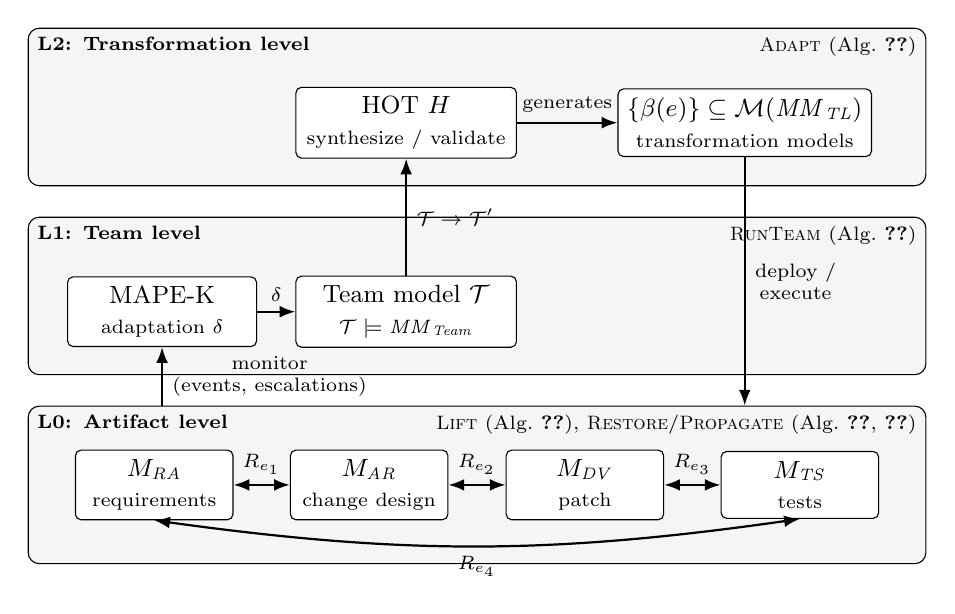
\begin{tikzpicture}[
  font=\small,
  lvl/.style={draw, rounded corners, fill=gray!8, minimum width=11.4cm,
              minimum height=2.0cm},
  mdl/.style={draw, rounded corners=2pt, fill=white, minimum width=2.0cm,
              minimum height=0.85cm, align=center},
  arr/.style={-{Latex[length=2mm]}, thick},
  bx/.style={{Latex[length=2mm]}-{Latex[length=2mm]}, thick},
  lab/.style={font=\scriptsize, align=center}
]
  \node[lvl] (L2) at (0,4.8) {};
  \node[lvl] (L1) at (0,2.4) {};
  \node[lvl] (L0) at (0,0)   {};
  \node[anchor=north west, font=\bfseries\scriptsize] at (L2.north west)
       {L2: Transformation level};
  \node[anchor=north west, font=\bfseries\scriptsize] at (L1.north west)
       {L1: Team level};
  \node[anchor=north west, font=\bfseries\scriptsize] at (L0.north west)
       {L0: Artifact level};
  \node[anchor=north east, font=\scriptsize] at (L0.north east)
       {\textsc{Lift} (Alg.~\ref{alg:lift}), \textsc{Restore}/\textsc{Propagate}
        (Alg.~\ref{alg:restore},~\ref{alg:prop})};
  \node[anchor=north east, font=\scriptsize] at (L1.north east)
       {\textsc{RunTeam} (Alg.~\ref{alg:run})};
  \node[anchor=north east, font=\scriptsize] at (L2.north east)
       {\textsc{Adapt} (Alg.~\ref{alg:adapt})};
  % L2
  \node[mdl, minimum width=2.8cm] (hot) at (-0.9,4.6)
       {HOT $H$\\{\scriptsize synthesize / validate}};
  \node[mdl, minimum width=3.2cm] (tms) at (3.4,4.6)
       {$\{\beta(e)\}\subseteq\Mods{\MM_{\TL}}$\\{\scriptsize transformation models}};
  \draw[arr] (hot) -- node[above, lab] {generates} (tms);
  % L1
  \node[mdl, minimum width=2.4cm] (mk) at (-4.0,2.2)
       {MAPE-K\\{\scriptsize adaptation $\delta$}};
  \node[mdl, minimum width=2.8cm] (tm) at (-0.9,2.2)
       {Team model $\team$\\{\scriptsize $\team\models\MM_{\Team}$}};
  \draw[arr] (mk) -- node[above, lab] {$\delta$} (tm);
  % L0
  \node[mdl] (ra) at (-4.1,0.0) {$M_{\mathit{RA}}$\\{\scriptsize requirements}};
  \node[mdl] (ar) at (-1.37,0.0) {$M_{\mathit{AR}}$\\{\scriptsize change design}};
  \node[mdl] (dv) at (1.37,0.0)  {$M_{\mathit{DV}}$\\{\scriptsize patch}};
  \node[mdl] (ts) at (4.1,0.0)   {$M_{\mathit{TS}}$\\{\scriptsize tests}};
  \draw[bx] (ra) -- node[above, lab] {$R_{e_1}$} (ar);
  \draw[bx] (ar) -- node[above, lab] {$R_{e_2}$} (dv);
  \draw[bx] (dv) -- node[above, lab] {$R_{e_3}$} (ts);
  \draw[bx] (ra.south) to[bend right=8] node[below, lab] {$R_{e_4}$} (ts.south);
  % cross-level
  \draw[arr] (tm) -- node[right, lab] {$\team\to\team'$} (hot);
  \draw[arr] (tms.south) -- node[right, lab, pos=0.5] {deploy /\\execute}
             (tms.south |- L0.north);
  \draw[arr] (mk.south |- L0.north) -- node[right, lab] {monitor\\(events, escalations)}
             (mk.south);
\end{tikzpicture}}
\caption{\tool{} at a glance on the running example. L0: agents' view models
related by consistency relations $R_e$; L1: the team as a runtime model
adapted by a MAPE-K loop; L2: higher-order transformations that (re)generate
the L0 relations whenever the team changes.}
\label{fig:overview}
\end{figure}

\smallskip\noindent\textbf{Research challenges.}
\RC{1}~\emph{Metamodeling open-ended agent knowledge:} agent artifacts mix
checkable structure with natural-language rationale; over-structuring removes
the flexibility that makes LLMs useful, under-structuring re-creates untyped
hand-offs.
\RC{2}~\emph{Consistency under stochastic transformations:} bx laws presuppose
deterministic, correct restorers; LLM restorers are stochastic and oracles err,
and consistency must hold over a \emph{network} of views where restoration
order matters~\cite{stevens2020networks,klare2023termination}.
\RC{3}~\emph{Runtime co-evolution of teams and transformations:} changing the
team changes the view metamodels and hence the transformations between
them~\cite{hebig2017coevolution}, which must be regenerated and validated while
the team runs.

\smallskip\noindent\textbf{Contributions.}
\begin{itemize}[leftmargin=*,nosep]
  \item A formalization of LLM team collaboration as a network of view models
  with hybrid consistency relations, an explicit oracle-error model, and a
  problem statement with four conditions (Sections~\ref{sec:background}
  and~\ref{sec:problem}).
  \item \tool{}: five interlocking algorithms with termination, run-invariant,
  \emph{structural} soundness, a \emph{probabilistic} semantic-error bound, and
  sound-adaptation guarantees (Section~\ref{sec:approach}).
  \item An evaluation on four SWE-bench-family benchmarks with seven
  pre-registered hypotheses, controlled baselines that isolate each mechanism,
  a second team design derived from prior work, and fidelity analyses of every
  LLM-backed component (Section~\ref{sec:evaluation}).
  \item A replication package with a map from every definition and algorithm to
  code (Section~\ref{sec:data}).
\end{itemize}



%=====================================================
%=====================================================
%=====================================================
%-------------------------[Background]----------------
%=====================================================
%=====================================================
%=====================================================



%=============================================================
\section{Background} \label{sec:background} %=============================================================

\subsection{Running Example} \label{subsec:example}

\begin{runbox}
\noindent\textbf{\devteam{}.} Four agents, modeled after the roles of
MAGIS~\cite{tao2024magis}, resolve a GitHub issue: a requirements analyst
($\mathit{RA}$) turns the issue into requirements and a reproduction scenario;
an architect ($\mathit{AR}$) localizes the fault and designs \emph{change
points}; a developer ($\mathit{DV}$) writes patch hunks; a tester
($\mathit{TS}$) writes and runs reproduction and regression tests. The edges
are $e_1{=}(\mathit{RA},\mathit{AR})$, $e_2{=}(\mathit{AR},\mathit{DV})$,
$e_3{=}(\mathit{DV},\mathit{TS})$, and $e_4{=}(\mathit{RA},\mathit{TS})$,
forming a cycle.

\smallskip\noindent\textbf{Issue (hypothetical).} ``\code{Duration.parse("1h30m")}
returns one hour; the minutes are silently dropped.''

\smallskip\noindent\textbf{What goes wrong without \tool{}.}
(P1)~The expected value ($5400$\,s) is lost when $\mathit{RA}$'s summary is
paraphrased for $\mathit{TS}$.
(P2)~After $\mathit{DV}$ fixes the parser, $\mathit{TS}$ finds that the
round trip \code{parse(str(d)) == d} breaks because \code{\_\_str\_\_} emits
\code{"1h30m0s"}. This finding is a \emph{new requirement}, but it reaches
$\mathit{DV}$ only as a chat message, and nothing links it to a requirement or
a design decision.
(P3)~A later regression in \code{report.py}, which no change point covers,
reveals that the team lacks impact analysis; adding an impact analyst
($\mathit{IA}$) would require re-wiring the team by hand.

\smallskip\noindent Section~\ref{sec:approach} resolves the issue in five
steps, \step{1}--\step{5}.
\end{runbox}

\subsection{LLM-Based Multi-Agent Systems} \label{subsec:mas}
An LLM agent couples an LLM with a role prompt, tools, and memory, and acts
iteratively. Multi-agent systems differ mainly in their communication
structure: fixed standard operating procedures with structured documents
(MetaGPT~\cite{hong2024metagpt}), chains of role-pair dialogues
(ChatDev~\cite{qian2024chatdev}), programmable conversations
(AutoGen~\cite{wu2024autogen}, CAMEL~\cite{li2023camel}), dynamic recruitment
(AgentVerse~\cite{chen2024agentverse}), and optimizable
graphs~\cite{zhuge2024gptswarm,hu2025adas,zhang2025aflow}. In issue
resolution, MAGIS splits the work among a manager, a repository custodian, a
developer, and a QA engineer~\cite{tao2024magis}. In all of them, the unit of
exchange is a message; the relation between different agents' working states
is implicit.

\subsection{Formal Foundations} \label{subsec:formal}

\noindent\textbf{Metamodels and models.} We use the graph-based view of
MDE~\cite{ehrig2006fundamentals}.

\begin{definition}[Metamodel]\label{def:mm}
A \emph{type graph} $\mathit{TG}=(C,\mathit{Ref},\mathit{Att},
\mathit{src},\mathit{tgt},\mathit{att},\sqsubseteq)$ has classes $C$,
references with $\mathit{src},\mathit{tgt}\colon\mathit{Ref}\to C$,
attributes with $\mathit{att}\colon\mathit{Att}\to C\times\mathbb{D}$ over data
types $\mathbb{D}$, and an inheritance order ${\sqsubseteq}$. A
\emph{metamodel} $\MM=(\mathit{TG},\Phi)$ adds well-formedness constraints
$\Phi$ (multiplicities, OCL invariants~\cite{omg2014ocl}). $\mathbb{D}$
contains a type $\NL$ of free text whose values constraints do not interpret.
\end{definition}

\begin{definition}[Model, conformance]\label{def:model}
A \emph{model} over $\MM$ is an instance graph $G=(O,L,\mathit{val})$ with
object identities $O$, links $L\subseteq O\times\mathit{Ref}\times O$, and an
attribute valuation, together with a typing $t\colon O\to C$ compatible with
$\mathit{src}$, $\mathit{tgt}$, and ${\sqsubseteq}$. We write
$\AllMods{\MM}$ for all models over $\MM$ and
$\Mods{\MM}=\{M\in\AllMods{\MM}\mid M\models\varphi\ \forall\varphi\in\Phi\}$
for the \emph{conforming} ones. A value of type $\NL$ may be the distinguished
\emph{hole} $\square$; a model without holes is \emph{complete}.
\end{definition}

Holes borrow the idea of partial models~\cite{famelis2012partial}: a model
with holes denotes the set of its completions.

\subsection{Consistency Relations and Transformation Networks}
\label{subsec:bx}
We follow the relational formulation of bx by Stevens~\cite{stevens2010qvt}.

\begin{definition}[Bidirectional transformation]\label{def:bx}
A bx between $\MM_a$ and $\MM_b$ is a triple $(R,\fwd{R},\bwd{R})$ with a
consistency relation $R\subseteq\Mods{\MM_a}\times\Mods{\MM_b}$ and restorers
$\fwd{R}\colon\Mods{\MM_a}\times\Mods{\MM_b}\to\Mods{\MM_b}$ and
$\bwd{R}\colon\Mods{\MM_a}\times\Mods{\MM_b}\to\Mods{\MM_a}$. It is
\emph{correct} if restoration yields consistent pairs and \emph{hippocratic}
if restorers return their input unchanged on consistent pairs.
\end{definition}

When several models are pairwise related, as in a team, the relations form a
\emph{transformation network}. Pairwise consistency need not imply a jointly
consistent state, and the result of restoration can depend on the execution
order~\cite{stevens2020networks}; Klare and Gleitze characterize the
termination and expressiveness of execution strategies for such
networks~\cite{klare2023termination}. View-based approaches such as
Vitruvius keep views consistent through explicit consistency
specifications~\cite{klare2021vitruvius}.

\begin{definition}[Higher-order transformation]\label{def:hot}
If transformations are models of a transformation-language metamodel
$\MM_{\TL}$, a \emph{HOT} is a transformation whose input or output models are
transformation models~\cite{tisi2009hot}.
\end{definition}

\subsection{Why Relational bx?} \label{subsec:why}
Four established alternatives exist; each conflicts with a property of agent
teams.
\emph{Lenses}~\cite{foster2007lenses} are asymmetric: one side must contain all
information of the other, whereas an architect and a tester hold
complementary information.
\emph{Triple graph grammars}~\cite{schurr1994tgg} derive restorers from
deterministic graph rules, which cannot express the $\NL$ content that LLMs
must produce; we use TGG-style rules only for the structural part.
\emph{Single-underlying-model} approaches, both in MDE~\cite{klare2021vitruvius}
and in agent systems~\cite{zhang2026patchboard}, derive every view from one
central model; with LLM agents that model must either fit into each agent's
context or be projected by yet another LLM, which reintroduces lossy hand-offs.
\emph{Uncertainty-aware bx}~\cite{eramo2015uncertainty} represent
alternative results explicitly, whereas our uncertainty is in the
\emph{correctness} of restorers and oracles.
Relational bx impose none of these commitments, and their laws can be weakened
precisely where LLMs are involved (Section~\ref{sec:problem}).

\subsection{Models at Runtime} \label{subsec:runtime}
A runtime model is causally connected to a running
system~\cite{blair2009runtime}; it serves as the knowledge of a MAPE-K loop
that monitors, analyzes, plans, and executes
adaptations~\cite{kephart2003autonomic,weyns2020sas}. When metamodels evolve,
models and transformations must co-evolve~\cite{hebig2017coevolution},
traditionally at design time.



%=============================================================
\section{Problem Formulation}\label{sec:problem}
%=============================================================

\begin{definition}[Agent]\label{def:agent}
An agent is $a=(\MM_a,\pi_a,\mathit{Cap}_a)$ with a view metamodel $\MM_a$, an
LLM-backed policy $\pi_a\colon\Mods{\MM_a}\times\mathit{Obl}\to\Dist{\Sigma^*}$
that maps the agent's model and its open obligations
(Definition~\ref{def:obl}) to a distribution over \emph{text} responses, and
capabilities $\mathit{Cap}_a$ (tools, back-end, cost). Its \emph{lifted
policy} is $\textsc{Lift}_a\circ\pi_a$ (Algorithm~\ref{alg:lift}).
\end{definition}

\begin{definition}[Team model]\label{def:team}
A team is $\team=(A,E,\beta,\omega)$ with agents $A$, edges $E\subseteq
A\times A$, a map $\beta\colon E\to\Mods{\MM_{\TL}}$ from edges to
transformation models, and propagation rights $\omega\colon
E\to\{\rightarrow,\leftarrow,\leftrightarrow\}$ stating which endpoint(s)
restoration may overwrite. The semantics of a transformation model is
$\den{\beta(e)}=(R_e,\fwd{R_e},\bwd{R_e},O_e)$: a bx plus an oracle. A team is
itself a model, $\team\in\Mods{\MM_{\Team}}$.
\end{definition}

\begin{definition}[Collaboration state]\label{def:state}
A state of $\team$ is $\sigma=(M_a,v_a)_{a\in A}$ with $M_a\in\Mods{\MM_a}$
and a version stamp $v_a\in\mathbb{N}$ incremented whenever $M_a$ changes. An
edge $e=(a,b)$ is \emph{checked-consistent} in $\sigma$ if
$(M_a,M_b)\in R_e^{\str}$ and $O_e(M_a,M_b)=1$ (Definition~\ref{def:hybrid}).
\end{definition}

\begin{definition}[Hybrid consistency and oracle error]\label{def:hybrid}
Each relation splits into $R_e=R_e^{\str}\cap R_e^{\sem}$, where $R_e^{\str}$
constrains only structure and non-$\NL$ attributes and is decidable, and
$R_e^{\sem}$ constrains $\NL$ content and is accessible only through an oracle
$O_e\colon\Mods{\MM_a}\times\Mods{\MM_b}\to\{0,1\}$ (a test execution or an
LLM judge). A call of $O_e$ on a pair $p$ is a \emph{false accept} if
$O_e(p)=1$ and $p\notin R_e^{\sem}$, and a \emph{false reject} if $O_e(p)=0$
and $p\in R_e^{\sem}$.
\end{definition}

\begin{assumption}[Serialized steps]\label{as:serial}
Agents act one at a time; each propagation has a single source of change.
\end{assumption}
\begin{assumption}[Bounded oracle error]\label{as:oracle}
For every call of $O_e$, conditioned on the history of the run, the
probability of a false accept is at most $\epsilon_e$ and of a false reject at
most $\rho_e$. The bound is over the distribution of candidates produced by the
restorers, so it applies to deterministic judges as well.
\end{assumption}
\begin{assumption}[Structural rules]\label{as:rules}
For each edge, a deterministic rule restorer $\mathit{Rule}_e$ exists such
that $(m,\mathit{Rule}_e(m,n))\in R_e^{\str}$, possibly with holes; empty
models are consistent: $(\emptyset,\emptyset)\in R_e$.
\end{assumption}

\begin{definition}[Obligations]\label{def:obl}
An obligation is a triple $(a,\kappa,x)$ assigning to agent $a$ a work item of
kind $\kappa\in\{\mathit{task},\mathit{hole},\mathit{escalation},
\mathit{failing}\}$ about element $x$: the initial task, a hole in $M_a$, an
escalated edge (Algorithm~\ref{alg:prop}), or a failing sub-goal of the
acceptance predicate $\varphi$. $\textsc{Schedule}$ picks the obligation with
the highest kind priority (escalation $>$ failing $>$ hole $>$ task), breaking
ties by a fixed agent order, so scheduling is deterministic.
\end{definition}

\begin{definition}[Adaptation]\label{def:adapt}
An adaptation is $(\delta,H,\mu)$: an endogenous transformation
$\delta\colon\Mods{\MM_{\Team}}\times K\to\Mods{\MM_{\Team}}$ driven by
monitored knowledge $K$; a HOT $H$ that yields $\beta'(e)$ for every new edge of
$\team'=\delta(\team,K)$; and a state migration $\mu$ from states of $\team$ to
states of $\team'$.
\end{definition}

\begin{definition}[Levels]\label{def:levels}
The \emph{hierarchy} of \tool{} is the chain
$\Mods{\MM_a}\xleftarrow{\ \beta\ }\Mods{\MM_{\TL}}\xleftarrow{\ H\ }
\Mods{\MM_{\Team}}$: L0 elements are view models; L1 is the team model, whose
$\beta$-elements are models of the L0 relations; L2 is the HOT $H$, which maps
L1 elements to L0 relations. Each level is a model of the level below it.
\end{definition}

\begin{problem}[Adaptive consistent collaboration]\label{prob:main}
Given a task with an acceptance predicate $\varphi$, agents with view
metamodels, an initial team $\team_0$, and a cost budget $B$, construct
transformation models $\beta$, a propagation strategy, and an adaptation
$(\delta,H,\mu)$ such that every run
$(\team_0,\sigma_0)\to(\team_1,\sigma_1)\to\cdots$ satisfies:
\textbf{C1} (conformance) $\team_i\in\Mods{\MM_{\Team}}$ and
$M^i_a\in\Mods{\MM_a}$;
\textbf{C2} (bounded restoration) after each agent step, within a bounded
number of restorer invocations, every edge is checked-consistent or explicitly
escalated, and the probability that a checked-consistent edge violates
$R_e^{\sem}$ is bounded;
\textbf{C3} (sound adaptation) adaptations leave retained agents' models and
trace links unchanged and establish C2 on new edges;
\textbf{C4} (effectiveness) the run reaches $\varphi$ within budget $B$ as
often as possible.
\end{problem}

C1--C3 are safety conditions addressing P1--P3; C4 is the usual objective.
The difficulty is to meet C1--C3 without sacrificing C4, since structure,
oracle calls, and rejected candidates cost tokens and time.



%=====================================================
%=====================================================
%=====================================================
%---------------------------[Approach]----------------
%=====================================================
%=====================================================
%=====================================================



\section{Description of Approach}\label{sec:approach}

\tool{} consists of five algorithms. \textsc{RunTeam}
(Algorithm~\ref{alg:run}) drives the MAPE-K loop over the team model; it
\emph{lifts} each agent response into a view model
(Algorithm~\ref{alg:lift}), \emph{propagates} the change through the team
(Algorithm~\ref{alg:prop}) by means of \emph{guarded restorers}
(Algorithm~\ref{alg:restore}), and \emph{adapts} the team when monitored events
call for it (Algorithm~\ref{alg:adapt}). We first describe what a team
designer writes (Section~\ref{subsec:authoring}) and then each algorithm, using
steps \step{1}--\step{5} of the running example.

\subsection{Authoring a Team}\label{subsec:authoring}
A team designer declares, for each agent, a view metamodel whose classes carry
\emph{concept annotations} from a small vocabulary (e.g.,
\emph{requirement}, \emph{code element}, \emph{test}); for each edge, the
structural relation $R_e^{\str}$, its rule restorer $\mathit{Rule}_e$, the
oracle $O_e$, and the rights $\omega(e)$; and a library $\Lambda$ of adaptation
rules. An edge without declared correspondences is unconstrained
($R_e$ is the full relation) and degrades gracefully to plain message
passing, so a team can be migrated to \tool{} edge by edge.

\smallskip\noindent\textbf{\devteam{} views.} $\MM_{\mathit{RA}}$:
\cls{Requirement} (id, kind, $\NL$ statement) and \cls{ReproScenario} (input,
expected, observed). $\MM_{\mathit{AR}}$: \cls{CodeElement} (path, symbol) and
\cls{ChangePoint} (target, realized requirement ids, $\NL$ rationale).
$\MM_{\mathit{DV}}$: \cls{Hunk} (path, range, diff, realized change point).
$\MM_{\mathit{TS}}$: \cls{TestCase} (kind \emph{repro}/\emph{regression}, code,
verified requirement ids, verdict, patch version) and \cls{Finding} ($\NL$).
Table~\ref{tab:corr} lists the relations. Wherever possible the oracle is
executable, which lowers $\epsilon_e$; $\omega$ encodes authority, e.g., a
developer may not change the design ($\omega(e_2)={\rightarrow}$), whereas
requirements and tests inform each other ($\omega(e_4)={\leftrightarrow}$).

\begin{table*}[t]
\centering
\caption{Consistency relations of \devteam{}. $R_e^{\str}$ is checked
deterministically; $R_e^{\sem}$ through the oracle $O_e$. Rows marked $\ast$
are synthesized at runtime by the HOT $H$ (Section~\ref{subsec:adapt}).}
\label{tab:corr}
\footnotesize
\begin{tabular}{@{}l c p{0.46\textwidth} p{0.30\textwidth}@{}}
\toprule
Edge & $\omega$ & Structural part $R_e^{\str}$ & Oracle $O_e$ for $R_e^{\sem}$ \\
\midrule
$e_1{=}(\mathit{RA},\mathit{AR})$ & $\leftrightarrow$ &
every \cls{Requirement} is realized by $\ge1$ \cls{ChangePoint}; change points
realize only existing requirements &
LLM judge: rationale addresses the requirement \\
$e_2{=}(\mathit{AR},\mathit{DV})$ & $\rightarrow$ &
every \cls{ChangePoint} is realized by $\ge1$ \cls{Hunk} in its target file;
every \cls{Hunk} realizes a \cls{ChangePoint} &
patch applies and builds; LLM judge: hunk implements rationale \\
$e_3{=}(\mathit{DV},\mathit{TS})$ & $\rightarrow$ &
every file touched by a \cls{Hunk} is covered by $\ge1$ selected regression
test; every verdict records the current patch version &
executable: verdicts obtained on current patch \\
$e_4{=}(\mathit{RA},\mathit{TS})$ & $\leftrightarrow$ &
every \cls{Requirement} is verified by $\ge1$ repro test; every authored test
verifies an existing requirement &
executable: repro test fails on original code; LLM judge: test encodes
requirement \\
$(\mathit{AR},\mathit{IA})^{\ast}$ & $\rightarrow$ &
every targeted \cls{CodeElement} has its callers listed as \cls{Dependency}
objects & executable: call-graph query \\
$(\mathit{IA},\mathit{TS})^{\ast}$ & $\rightarrow$ &
every impacted module is covered by $\ge1$ selected regression test &
executable: verdicts on current patch \\
\bottomrule
\end{tabular}
\end{table*}

\subsection{Orchestration}\label{subsec:run}
Algorithm~\ref{alg:run} keeps $\team$ and $\sigma$ as runtime models (L1). An
agent's response enters the team \emph{only} through \textsc{Lift} and
\textsc{Propagate} (lines~\ref{ln:run-lift}--\ref{ln:run-prop}); there is no
side channel of free-text messages. The run ends when $\varphi$ holds or the
budget is spent; in both cases the artifact is produced by a model-to-text
transformation (line~\ref{ln:run-ret}), so a best-effort patch is always
submitted.

\begin{algorithm}[t]
\caption{\textsc{RunTeam}: orchestration (L1)}\label{alg:run}
\small
\begin{algorithmic}[1]
\Input task $x$; team $\team_0$; acceptance predicate $\varphi$; budget $B$
\Output artifact $\textsc{M2T}(\sigma)$ and flag $\varphi(\sigma)$
\State $\team\gets\team_0$;\; $\sigma\gets(\emptyset,0)_{a\in A}$;\;
       $K,X\gets\emptyset$;\; $\mathit{Obl}\gets\{(a_0,\mathit{task},x)\}$
\While{$\neg\varphi(\sigma)$ \textbf{and} $\mathit{cost}<B$}\label{ln:run-loop}
  \State $(a,o)\gets\textsc{Schedule}(\mathit{Obl})$
         \Comment{Def.~\ref{def:obl}}
  \State $r\gets$ sample of $\pi_a(M_a,o)$ \Comment{LLM turn with tools}
  \State $(M',\Delta)\gets\textsc{Lift}(r,\MM_a,M_a)$
         \Comment{Alg.~\ref{alg:lift}}\label{ln:run-lift}
  \If{$M'=\bot$} $K\gets K\cup\{\mathit{liftFail}(a)\}$
  \Else
    \State $M_a\gets M'$;\; $v_a\gets v_a+1$
    \State $(\sigma,X)\gets\textsc{Propagate}(\team,\sigma,\{a\},X,\omega)$
           \Comment{Alg.~\ref{alg:prop}}\label{ln:run-prop}
    \State $K\gets K\cup\textsc{Events}(a,\Delta,X)$
  \EndIf
  \State $(\team,\sigma,X)\gets\textsc{Adapt}(\team,\sigma,K,X)$
         \Comment{Alg.~\ref{alg:adapt}}\label{ln:run-adapt}
  \State $\mathit{Obl}\gets\textsc{Obligations}(\team,\sigma,X,\varphi)$
\EndWhile
\State \Return $(\textsc{M2T}(\sigma),\varphi(\sigma))$\label{ln:run-ret}
\end{algorithmic}
\end{algorithm}

\subsection{Lifting Agent Output}\label{subsec:lift}
Algorithm~\ref{alg:lift} addresses the receiving side of P1: whatever an agent
produces must be a conforming model of its view before anyone else sees it. It
derives a JSON schema from $\MM_a$, decodes the response against it, checks
$\Phi_a$, and lets the agent repair violations up to $k_L$ times.
\textsc{Instantiate} reuses the identities of unchanged objects, so that trace
links survive iterations (P2). Lift is itself LLM-dependent; we therefore
measure its fidelity separately (RQ5).

\begin{algorithm}[t]
\caption{\textsc{Lift}: response to conforming view model (L0)}
\label{alg:lift}
\small
\begin{algorithmic}[1]
\Input response $r$; $\MM_a=(\mathit{TG}_a,\Phi_a)$; current $M$; retries $k_L$
\Output $(M',\textsc{Diff}(M,M'))$ with $M'\in\Mods{\MM_a}$, or $\bot$
\State $S\gets\textsc{Schema}(\MM_a)$
\For{$j=1$ \textbf{to} $k_L$}
  \State $M'\gets\textsc{Instantiate}(\textsc{Decode}(r,S),\mathit{TG}_a,M)$
         \Comment{stable ids}
  \State $V\gets\textsc{TypeErrors}(M')\cup\{\phi\in\Phi_a\mid M'\not\models\phi\}$
  \If{$V=\emptyset$} \Return $(M',\textsc{Diff}(M,M'))$ \EndIf
  \State $r\gets\pi_a.\textsc{Repair}(r,\textsc{Explain}(V))$
\EndFor
\State \Return $\bot$
\end{algorithmic}
\end{algorithm}

\smallskip\noindent\step{1}\,$\mathit{RA}$ reads the issue; \textsc{Lift}
yields requirement $r_1$ (``\code{parse} honors every component'') and
scenario $s_1$ (input \code{"1h30m"}, expected $5400$, observed $3600$). A
first response that omitted the expected value violates the multiplicity of
\cls{ReproScenario.expected} and is repaired, so the value cannot be lost
downstream (P1).

\subsection{Guarded Hybrid Restoration}\label{subsec:restore}
Algorithm~\ref{alg:restore} restores one edge in one direction. A
deterministic rule first repairs the structure and opens holes
(Assumption~\ref{as:rules}); an LLM fills \emph{only} the holes; a candidate is
accepted only if it conforms, satisfies $R_e^{\str}$, and passes $O_e$.
Rejection diagnoses are fed back to the next attempt.

\begin{algorithm}[t]
\caption{\textsc{GuardedRestore}: one edge, one direction (L0)}
\label{alg:restore}
\small
\begin{algorithmic}[1]
\Input edge $e$; source model $m$; target model $n$; attempts $k$
\Output $n'$ with $(m,n')$ checked-consistent, or $(\bot,D)$
\If{$(m,n)\in R_e^{\str}$ \textbf{and} $O_e(m,n)=1$} \Return $n$
   \label{ln:rest-hip}\EndIf
\State $n_0\gets\mathit{Rule}_e(m,n)$;\; $D\gets\emptyset$
       \Comment{structure fixed; holes open}
\For{$j=1$ \textbf{to} $k$}
  \State $n'\gets\textsc{FillHoles}(e,m,n_0,D)$
         \Comment{LLM; identity if no holes}
  \If{$n'\in\Mods{\MM_t}$ \textbf{and} $(m,n')\in R_e^{\str}$ \textbf{and}
      $O_e(m,n')=1$} \Return $n'$ \EndIf
  \State $D\gets D\cup\textsc{Diagnose}(e,m,n')$
\EndFor
\State \Return $(\bot,D)$
\end{algorithmic}
\end{algorithm}

\smallskip\noindent\step{2}\,Propagating \step{1} along $e_4$,
$\mathit{Rule}_{e_4}$ creates a repro test $t_1$ verifying $r_1$ whose body is
a hole; the LLM fills it with \code{parse("1h30m").seconds == 5400}; the
executable oracle confirms that $t_1$ fails on the original code, as a
reproduction test must. Along $e_1$, $\mathit{Rule}_{e_1}$ creates a change
point $cp_1$ whose target and rationale are holes, i.e., obligations of
$\mathit{AR}$.

\subsection{Propagation Through the Team}\label{subsec:prop}
Algorithm~\ref{alg:prop} restores consistency over the network (\RC{2}). The
worklist $W$ is a priority queue over a fixed edge order, which makes runs
reproducible. For an edge that is not checked-consistent, it overwrites the
endpoint with the \emph{older} version stamp, provided $\omega'$ permits it;
ties go to the endpoint $\omega'$ permits, and to the edge's target if both are
permitted. If $\omega'$ forbids the direction, the change itself is
illegitimate and is escalated to its author. The per-edge budget $\ell$ bounds
work on cycles.

\begin{algorithm}[t]
\caption{\textsc{Propagate}: consistency over the network (L0)}
\label{alg:prop}
\small
\begin{algorithmic}[1]
\Input $\team=(A,E,\beta,\omega)$; $\sigma$; changed agents $C$;
escalations $X_0$; rights $\omega'$; budget $\ell$
\Output $(\sigma,X)$
\State $W\gets\{e\in E\mid e\cap C\neq\emptyset\}\cup\mathit{edges}(X_0)$;\;
       $X\gets\emptyset$;\; $u[\cdot]\gets0$
\While{$W\neq\emptyset$}
  \State $e=(a,b)\gets\textsc{PopMin}(W)$
  \If{$e$ is checked-consistent in $\sigma$} \textbf{continue}\label{ln:prop-ok}
  \EndIf
  \State $t\gets\textsc{Direction}(e,\sigma,\omega')$
         \Comment{older stamp; $\bot$ if forbidden}
  \If{$t=\bot$ \textbf{or} $u[e]\ge\ell$}
    \State $X\gets X\cup\{\textsc{Diagnose}(e,\sigma)\}$;\;\textbf{continue}
  \EndIf
  \State $u[e]\gets u[e]+1$;\;
         $n'\gets\textsc{GuardedRestore}(e\to t,\sigma,k)$
  \If{$n'=(\bot,D)$} $X\gets X\cup\{(e,D)\}$;\;\textbf{continue}\EndIf
  \If{$n'\neq M_t$}
    \State $M_t\gets n'$;\; $v_t\gets v_t+1$
    \State $W\gets W\cup\{e'\in E\setminus\{e\}\mid t\in e'\}$
           \label{ln:prop-enq}
  \EndIf
\EndWhile
\State \Return $(\sigma,X)$
\end{algorithmic}
\end{algorithm}

Let $d_e$ be the number of other edges sharing an endpoint with $e$.

\begin{proposition}[Termination]\label{prop:term}
\textsc{Propagate} performs at most $\ell|E|$ restorations and terminates.
\end{proposition}
\noindent\emph{Sketch.} Each restoration increments some $u[e]\le\ell$; other
iterations shrink $W$; edges are added only after a restoration
(line~\ref{ln:prop-enq}). \hfill$\square$

\begin{lemma}[Postcondition and run invariant]\label{lem:inv}
On return of \textsc{Propagate}, every edge is checked-consistent or in
$\mathit{edges}(X)$, provided this held before the call for all edges not
incident to $C$. Hence, after every iteration of \textsc{RunTeam}, every edge
is checked-consistent or escalated.
\end{lemma}
\noindent\emph{Sketch.} Invariant: every edge not checked-consistent since the
last change of its endpoints is in $W$ or $X$. A restoration makes $e$
checked-consistent and re-enqueues all other edges at the changed endpoint.
The run-level claim follows by induction, using $(\emptyset,\emptyset)\in R_e$
(Assumption~\ref{as:rules}) and Proposition~\ref{prop:adapt} for adaptation
steps. \hfill$\square$

\begin{corollary}[Structural soundness]\label{cor:sound}
If \textsc{Propagate} returns $X=\emptyset$, all models conform and all edges
satisfy $R_e^{\str}$ and their oracles.
\end{corollary}

\begin{proposition}[Semantic error bound]\label{prop:sem}
Let $N_e$ be the number of oracle calls on $e$ during one call of
\textsc{Propagate}; then $N_e\le 1+\ell d_e+(k+1)\ell$. Under
Assumption~\ref{as:oracle}, the probability that \textsc{Propagate} returns
$X=\emptyset$ while some edge violates $R_e^{\sem}$ is at most
$\sum_{e\in E}\epsilon_e\,\mathbb{E}[N_e]$.
\end{proposition}
\noindent\emph{Sketch.} $e$ is enqueued initially and after each change of an
endpoint by an adjacent restoration ($\le\ell d_e$); each pop costs one call
and each own restoration at most $k{+}1$. If $e$ ends semantically
inconsistent, the last call on $e$ accepted exactly the final pair, since
later endpoint changes would re-enqueue $e$; that call was a false accept. By
Assumption~\ref{as:oracle}, the expected number of false accepts is at most
$\sum_e\epsilon_e\mathbb{E}[N_e]$, which bounds the probability.
\hfill$\square$

The bound grows with retries: every retry is another chance to accept a wrong
candidate. This is why an edge's budgets $k$ and $\ell$ trade effectiveness
against semantic risk, and why executable oracles (small $\epsilon_e$) matter.

\begin{remark}[Stability]
Line~\ref{ln:rest-hip} of Algorithm~\ref{alg:restore} and
line~\ref{ln:prop-ok} of Algorithm~\ref{alg:prop} make restoration hippocratic
only up to false rejects: a consistent edge is needlessly restored with
probability at most $\rho_e$ per check. Results may differ under other edge
orders, as in any transformation network~\cite{stevens2020networks}; the fixed
order makes each run reproducible, and RQ5 measures the effect of order.
\end{remark}

\smallskip\noindent\step{3}\,$\mathit{AR}$ localizes $cp_1$ to
\code{Duration.parse} in \code{duration.py}; along $e_2$ a hunk obligation opens for
$\mathit{DV}$, who rewrites the parsing expression ($h_1$). Along $e_3$ the
restorer re-runs the selected tests: $t_1$ passes, but
\code{test\_str\_roundtrip} fails.
\step{4}\,$\mathit{TS}$ records a finding and authors a round-trip test $t_2$.
Since $t_2$ verifies no requirement, $e_4$ is inconsistent, $t$ is
$\mathit{RA}$ (older stamp, $\omega(e_4)={\leftrightarrow}$), and restoration
runs \emph{backward}: $\mathit{Rule}_{e_4}$ creates $r_2$ with a hole that the
LLM fills and the judge accepts. The change re-enqueues $e_1$, which creates
$cp_2$ at \code{\_\_str\_\_}. The finding travels along explicit
correspondences, and the trace $t_2\to r_2\to cp_2$ records why $cp_2$ exists
(P2). When $\mathit{DV}$ later adds a hunk in \code{format.py} that realizes no
change point, $\omega(e_2)$ forbids changing the design from the patch side,
so the hunk is escalated to $\mathit{DV}$ instead of silently entering the
solution (P1).

\subsection{Runtime Adaptation}\label{subsec:adapt}
Algorithm~\ref{alg:adapt} closes the MAPE-K loop (P3, \RC{3}). Each rule
$\lambda=(\mathit{cond}_\lambda,\delta_\lambda)\in\Lambda$ pairs a condition
over monitored events with an endogenous team transformation, e.g.,
\emph{insert-impact-analyst} (regressions outside every change point occur
$\theta$ times), \emph{switch-back-end} (lift failures of an agent exceed a
threshold), and \emph{split-role}. At most $A_{\max}$ adaptations are applied
per run.

\begin{definition}[HOT $H$]\label{def:H}
Let $\gamma_a\colon C_a\to\mathcal{K}$ annotate classes with concepts, and let
a template library $\Theta$ map concept pairs to rule schemas, each with a
structural rule and an oracle kind. For a new edge $e=(a,b)$,
$H(\team',e)$ composes the instances of $\Theta(\gamma_a(c),\gamma_b(c'))$ for
all class pairs $(c,c')$ with a template. An LLM is used only to phrase the
prompts of judge oracles. \textsc{Validate} checks that $\beta'(e)$ type-checks
against $\MM_a$ and $\MM_b$ and that $\mathit{Rule}_e$ terminates with a
conforming model on the current $M_a$.
\end{definition}

\begin{algorithm}[t]
\caption{\textsc{Adapt}: MAPE-K with HOT synthesis (L1--L2)}
\label{alg:adapt}
\small
\begin{algorithmic}[1]
\Input $\team,\sigma,K,X$; rules $\Lambda$; HOT $H$; cap $A_{\max}$
\Output $(\team',\sigma',X')$
\If{$n_{\mathit{ad}}\ge A_{\max}$} \Return $(\team,\sigma,X)$\EndIf
\For{$\lambda\in\Lambda$ \textbf{by priority}}
  \If{$\mathit{cond}_\lambda(K,\team)$} \Comment{monitor, analyze}
    \State $r\gets\textsc{Try}(\lambda,\team,\sigma,X)$
    \If{$r\neq\bot$} $n_{\mathit{ad}}\gets n_{\mathit{ad}}+1$;\;
       $K\gets K\setminus\textsc{Consumed}(\lambda)$;\;\Return $r$\EndIf
    \State $K\gets K\cup\{\mathit{rejected}(\lambda)\}$ \Comment{roll back}
  \EndIf
\EndFor
\State \Return $(\team,\sigma,X)$
\Statex
\Function{Try}{$\lambda,\team,\sigma,X$}
  \State $\team'\gets\delta_\lambda(\team)$;\;
         \textbf{if} $\team'\notin\Mods{\MM_{\Team}}$ \textbf{return} $\bot$
  \State $N\gets$ edges of $\team'$ that are new or have a changed endpoint view
  \For{$e\in N$} \Comment{plan (L2)}
    \State $\beta'(e)\gets H(\team',e)$;\;
           \textbf{if} $\neg\textsc{Validate}(\beta'(e),\sigma)$
           \textbf{return} $\bot$
  \EndFor
  \State $\sigma'\gets\mu(\sigma,\team,\team')$ \Comment{copy retained models, ids, traces}
  \State $(\sigma',X')\gets\textsc{Propagate}(\team',\sigma',A'{\setminus}A,X,
         \omega_{\mathit{init}})$
  \State \textbf{if} $\mathit{edges}(X')\cap N\neq\emptyset$ \textbf{return}
         $\bot$ \textbf{else return} $(\team',\sigma',X')$
\EndFunction
\end{algorithmic}
\end{algorithm}

Here $\omega_{\mathit{init}}$ permits overwriting \emph{only} models of new
agents during initialization.

\begin{proposition}[Sound adaptation]\label{prop:adapt}
If \textsc{Adapt} returns $\team'\neq\team$, then $\team'\in
\Mods{\MM_{\Team}}$, the models and trace links of retained agents are
unchanged, and every edge in $N$ is checked-consistent (condition C3).
\end{proposition}
\noindent\emph{Sketch.} $\mu$ copies retained models with their identities;
$\omega_{\mathit{init}}$ forbids overwriting them; conformance and
consistency of $N$ are checked explicitly, otherwise $\textsc{Try}$ returns
$\bot$. \hfill$\square$

\begin{proposition}[Run termination]\label{prop:runterm}
If every agent turn costs at least $c_{\min}>0$, \textsc{RunTeam} performs at
most $\lceil B/c_{\min}\rceil$ iterations and at most $A_{\max}$ adaptations,
and terminates.
\end{proposition}

\smallskip\noindent\step{5}\,After $cp_2$ is fixed, a regression appears in
\code{report.py}, which no change point targets; as the second such event, it
triggers \emph{insert-impact-analyst}. $\delta$ adds $\mathit{IA}$ with
$\MM_{\mathit{IA}}$ (\cls{Dependency}, \cls{ImpactedModule}) and edges
$(\mathit{AR},\mathit{IA})$ and $(\mathit{IA},\mathit{TS})$. Because
\cls{CodeElement} and \cls{Dependency} are both annotated \emph{code element},
$H$ instantiates a call-graph template, yielding the last two rows of
Table~\ref{tab:corr}. $\mu$ keeps the four existing models verbatim and
initializes $M_{\mathit{IA}}$, which lists \code{report.py} as a caller of
\code{parse}. $\mathit{AR}$ adds $cp_3$, $\mathit{DV}$ patches it, and
$\varphi$ holds: both requirements are traced to passing repro tests and no
regression test fails. The team changed shape mid-run without re-wiring (P3).

\subsection{Complexity and Scalability}\label{subsec:complexity}
Let $c_{\mathit{LLM}}$ and $c_O$ be the costs of one hole-filling call and one
oracle call. By Propositions~\ref{prop:term} and~\ref{prop:sem}, one
propagation costs at most
$\ell|E|\,k\,c_{\mathit{LLM}}+\sum_e(1+\ell d_e+(k{+}1)\ell)\,c_O$, i.e.,
$O(|E|\,(k\,c_{\mathit{LLM}}+d_{\max}c_O))$ for fixed $\ell$. Unlike
approaches that explore the interleavings of agent
behaviors, \tool{} checks only the \emph{current} state, so there is no
state-space explosion; cost grows linearly in the number of edges, which
designers keep sparse. RQ6 measures the constants empirically.


%=====================================================
%=====================================================
%=====================================================
%-------------------------[Evaluation]----------------
%=====================================================
%=====================================================
%=====================================================

%=============================================================
\section{Evaluation}\label{sec:evaluation}
%=============================================================
% AUTHOR NOTE: red --.- (\ph) marks an unmeasured value; blue text (\hyp)
% marks a result-dependent sentence to be confirmed or rewritten; plots show
% placeholder data until \placeholderdatafalse is set.

We evaluate \tool{} on repository-level issue resolution through six research
questions.
\textbf{RQ1} (effectiveness) asks whether \tool{} resolves more issues than
single-agent, pipeline, and multi-agent approaches.
\textbf{RQ2} (collaboration) examines whether it reduces lossy hand-offs,
stale decisions, and inter-agent misalignment.
\textbf{RQ3} (mechanisms) measures the contribution of each mechanism.
\textbf{RQ4} (adaptation) tests runtime adaptation under perturbations.
\textbf{RQ5} (fidelity and guarantees) measures the fidelity of every
LLM-backed component and the error rates behind Proposition~\ref{prop:sem}.
\textbf{RQ6} (cost and scalability) measures cost and scaling with team size.

%=============================================================
\subsection{Experimental Setup}\label{subsec:setup}
%=============================================================

\subsubsection{Pre-registered hypotheses}
Table~\ref{tab:hyp} lists seven hypotheses, their tests, and success criteria.
They were fixed, together with the analysis scripts, before any evaluation run
and are time-stamped in the artifact \fixme{register, e.g., on OSF, before
running}. We report every outcome, including failures.

\begin{table}[t]
\centering
\caption{Pre-registered hypotheses (Holm-corrected, $\alpha=0.05$).}
\label{tab:hyp}
\footnotesize
\setlength{\tabcolsep}{2.5pt}
\begin{tabular}{@{}l p{0.52\columnwidth} p{0.33\columnwidth}@{}}
\toprule
ID & Hypothesis & Test \\
\midrule
H1 & \tool{} resolves more instances than \textsc{DevTeam-NL} on Verified and Pro &
paired GLMM, per run \\
H2 & The advantage grows with the number of files in the gold patch &
interaction term in H1's GLMM \\
H3 & \textsc{MAGIS-M2M} resolves more instances than MAGIS & paired GLMM \\
H4 & \tool{} lowers the share of inter-agent misalignment failures &
$\chi^2$ on MAST labels \\
H5 & Removing backward restoration lowers the resolve rate on Pro &
paired GLMM \\
H6 & Adaptive beats fixed teams in S1 and S3, with zero C3 violations &
paired GLMM; count \\
H7 & Executable oracles have lower $\epsilon_e$ than LLM judges &
two-proportion test \\
\bottomrule
\end{tabular}
\end{table}

\subsubsection{Benchmarks}
\emph{SWE-bench Lite}~\cite{jimenez2024swebench} (300 instances) enables
comparison with prior work; we also report its subset Lite-S, which excludes
instances with insufficient or misleading issue
descriptions~\cite{xia2025agentless}.
\emph{SWE-bench Verified}~\cite{openai2024verified} (500 instances) was
validated by human annotators.
\emph{SWE-bench-Live}~\cite{zhang2025swebenchlive} is curated automatically
from GitHub issues created since 2024, each with its own Docker image; we use
the \fixme{N} instances created after the training cut-off of our back-end.
\emph{SWE-Bench Pro}~\cite{deng2025swebenchpro} contains human-verified,
long-horizon tasks that often require multi-file patches; we use its public
set. Live and Pro constitute our contamination-resistant subset, which we
analyze separately.

\subsubsection{Development/test separation}
To prevent the team design from encoding the benchmark, all view metamodels,
correspondence rules, oracles, adaptation rules, templates, and prompts were
developed on \fixme{N} instances from the SWE-bench training split, whose
repositories are disjoint from all evaluation sets, and frozen at a tagged
commit \fixme{hash} before the first evaluation run. No evaluation instance was
inspected during development.

\subsubsection{Team designs}
Besides \devteam{}, we derive \textsc{MAGIS-M2M} by re-expressing the four
published roles of MAGIS~\cite{tao2024magis} as view metamodels with
correspondences, keeping MAGIS's prompts and workflow. Since we did not design
MAGIS's roles, \textsc{MAGIS-M2M} tests whether \tool{} benefits a team
structure chosen by others (H3).

\subsubsection{Baselines}
Single-agent: SWE-agent~\cite{yang2024sweagent} and
OpenHands~\cite{wang2025openhands}. Pipeline:
Agentless~\cite{xia2025agentless}. Multi-agent: MAGIS~\cite{tao2024magis}.
Controlled variants sharing \devteam{}'s agents, prompts, tools, and back-end:
\textsc{DevTeam-NL} (natural-language hand-offs);
\textsc{DevTeam-Typed} (every hand-off is a lifted, schema-valid message, but
there are no correspondences, propagation, or adaptation); and
\textsc{DevTeam-Schema} (one shared schema-validated state in the style
of~\cite{zhang2026patchboard}). The chain NL $\to$ Typed $\to$ \tool{}
separates the effect of typed outputs from that of correspondence-based
propagation.

\subsubsection{Protocol}
All systems use the same back-end (\fixme{model, version, date}), temperature
\fixme{T}, and per-instance budget \fixme{\$}, including all restorer and
oracle calls. Every system submits its final patch, whether or not its
internal checks pass. Agents never see the hidden evaluation tests; oracles use
only tests present before the fix. Each configuration runs three times.

\subsubsection{Metrics and statistics}
We report the official resolve rate. Following Arcuri and
Briand~\cite{arcuri2011practical}, we analyze per-run, per-instance outcomes
with generalized linear mixed models (logit link, random intercepts for
instance and repository), correct with Holm--Bonferroni, and report odds ratios
with 95\% bootstrap confidence intervals. RQ2--RQ5 metrics are defined in
their subsections.

\subsubsection{Implementation}
\tool{} is implemented in \fixme{Python, N\,kLOC}; view and team metamodels in
Ecore~\cite{steinberg2008emf} \fixme{via PyEcore}; constraints in
\fixme{OCL layer}; rule restorers as TGG-style rules in \fixme{internal DSL};
agents use SWE-agent's tool set~\cite{yang2024sweagent}. Parameters:
$k_L{=}\fixme{3}$, $k{=}\fixme{3}$, $\ell{=}\fixme{4}$, $\theta{=}\fixme{2}$,
$A_{\max}{=}\fixme{3}$, all fixed during development.

%=============================================================
\subsection{RQ1: Effectiveness}\label{subsec:rq1}
%=============================================================

\noindent\textbf{Methodology.} We compare resolve rates on all four benchmarks
(H1, H3) and model the effect of patch size (H2) with the number of files in
the gold patch as a covariate.

\noindent\textbf{Results.} Table~\ref{tab:main} and Fig.~\ref{fig:byfiles}.
\hyp{H1 is [supported / not supported]: \tool{} resolves \ph\% (Verified) and
\ph\% (Pro) vs.\ \ph\% and \ph\% for \textsc{DevTeam-NL} (OR $=\ph$,
95\% CI [\ph, \ph]).} \hyp{H2: the interaction coefficient is \ph\
($p=\ph$).} \hyp{H3: \textsc{MAGIS-M2M} vs.\ MAGIS, OR $=\ph$.}
\hyp{On the contamination-resistant subset, the ranking is [preserved / not
preserved].}

\begin{table*}[t]
\centering
\caption{RQ1: Resolved instances (\%, mean of three runs) and mean cost per
instance under a shared back-end and budget.}
\label{tab:main}
\footnotesize
\begin{tabular}{@{}l l r r r r r r r@{}}
\toprule
System & Type & Lite & Lite-S & Verified & Live & Pro & Cost (\$) & Tokens (k) \\
\midrule
SWE-agent~\cite{yang2024sweagent}  & single agent & \ph & \ph & \ph & \ph & \ph & \ph & \ph \\
OpenHands~\cite{wang2025openhands} & single agent & \ph & \ph & \ph & \ph & \ph & \ph & \ph \\
Agentless~\cite{xia2025agentless}  & pipeline     & \ph & \ph & \ph & \ph & \ph & \ph & \ph \\
MAGIS~\cite{tao2024magis}          & multi-agent  & \ph & \ph & \ph & \ph & \ph & \ph & \ph \\
\textsc{MAGIS-M2M}                 & multi-agent  & \ph & \ph & \ph & \ph & \ph & \ph & \ph \\
\textsc{DevTeam-NL}                & multi-agent  & \ph & \ph & \ph & \ph & \ph & \ph & \ph \\
\textsc{DevTeam-Typed}             & multi-agent  & \ph & \ph & \ph & \ph & \ph & \ph & \ph \\
\textsc{DevTeam-Schema}            & multi-agent  & \ph & \ph & \ph & \ph & \ph & \ph & \ph \\
\midrule
\tool{} (\devteam{})               & multi-agent  & \ph & \ph & \ph & \ph & \ph & \ph & \ph \\
\bottomrule
\end{tabular}
\end{table*}

\begin{figure}[t]
\centering
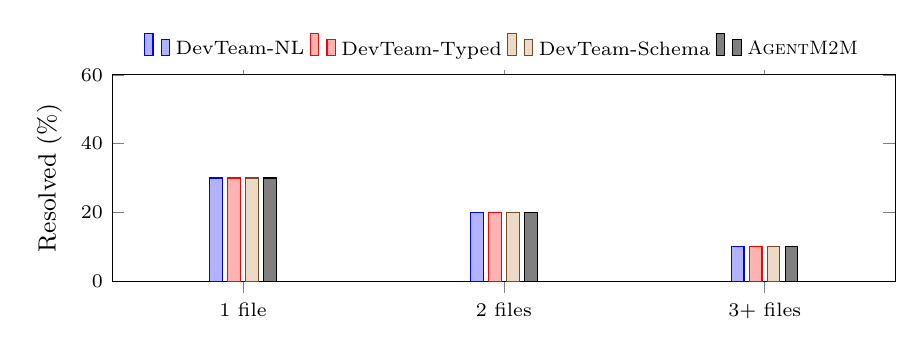
\begin{tikzpicture}
\begin{axis}[
  ybar, width=0.95\columnwidth, height=4.2cm, bar width=4.5pt,
  ymin=0, ymax=60, ylabel={Resolved (\%)}, ylabel style={font=\small},
  symbolic x coords={1 file,2 files,3+ files}, xtick=data,
  tick label style={font=\scriptsize},
  legend style={font=\scriptsize, at={(0.5,1.02)}, anchor=south,
                legend columns=4, draw=none},
  enlarge x limits=0.25]
% PLACEHOLDER DATA
\addplot coordinates {(1 file,30) (2 files,20) (3+ files,10)};
\addplot coordinates {(1 file,30) (2 files,20) (3+ files,10)};
\addplot coordinates {(1 file,30) (2 files,20) (3+ files,10)};
\addplot coordinates {(1 file,30) (2 files,20) (3+ files,10)};
\legend{DevTeam-NL, DevTeam-Typed, DevTeam-Schema, \tool{}}
\phwatermark
\end{axis}
\end{tikzpicture}
\caption{RQ1/H2: Resolve rate by number of files in the gold patch
(Verified and Pro).}
\label{fig:byfiles}
\end{figure}

\finding{\hyp{[State H1--H3 outcomes in one sentence each.]}}

%=============================================================
\subsection{RQ2: Collaboration Quality}\label{subsec:rq2}
%=============================================================
\noindent\textbf{Methodology.} On a stratified sample of \fixme{100}
instances, two authors independently annotated the requirements and facts
(expected values, API names, constraints) in each issue ($\kappa=\ph$). For
\emph{every} system we render each agent turn's complete input context---chat
messages or view models---as text, so that all metrics are measured on the same
kind of object: \emph{hand-off loss} (annotated facts absent from the context of
an agent that needs them), \emph{requirement coverage} (requirements addressed
by the final patch and tests), \emph{out-of-scope edits} (patched files not in
the gold patch), and \emph{stale decisions} (turns acting on verdicts of an
older patch). Failed runs are labeled with the MAST
LLM-as-a-judge~\cite{cemri2025mast} on the same renderings; because the judge
was validated on conversational traces, we re-validate it on \fixme{60} traces
per system against two human annotators ($\kappa=\ph$).

\noindent\textbf{Results.} Table~\ref{tab:collab}, Fig.~\ref{fig:mast}.
\hyp{H4 is [supported / not supported]: the inter-agent misalignment share
changes from \ph\% (\textsc{DevTeam-NL}) to \ph\% (\tool{}), $\chi^2=\ph$.}

\begin{table}[t]
\centering
\caption{RQ2: Collaboration metrics on the annotated sample.}
\label{tab:collab}
\footnotesize
\setlength{\tabcolsep}{3pt}
\begin{tabular}{@{}l r r r r@{}}
\toprule
Metric & NL & Typed & Schema & \tool{} \\
\midrule
Hand-off loss (\%) $\downarrow$        & \ph & \ph & \ph & \ph \\
Requirement coverage (\%) $\uparrow$   & \ph & \ph & \ph & \ph \\
Out-of-scope edits (\%) $\downarrow$   & \ph & \ph & \ph & \ph \\
Stale decisions / inst.\ $\downarrow$  & \ph & \ph & \ph & \ph \\
\bottomrule
\end{tabular}
\end{table}

\begin{figure}[t]
\centering
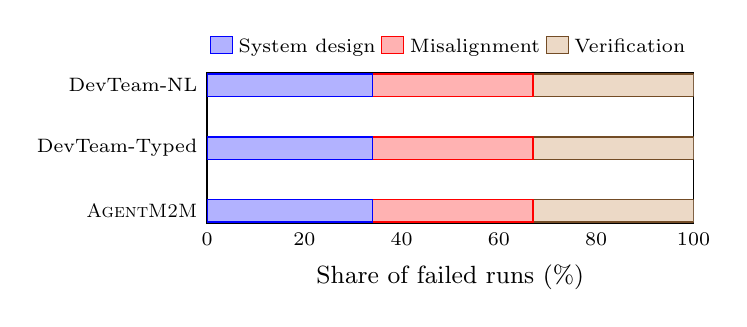
\begin{tikzpicture}
\begin{axis}[
  xbar stacked, width=0.64\columnwidth, height=3.5cm, bar width=8pt,
  xmin=0, xmax=100, xlabel={Share of failed runs (\%)},
  xlabel style={font=\small},
  symbolic y coords={\tool{},DevTeam-Typed,DevTeam-NL}, ytick=data,
  tick label style={font=\scriptsize},
  legend style={font=\scriptsize, at={(0.5,1.03)}, anchor=south,
                legend columns=3, draw=none}]
% PLACEHOLDER DATA
\addplot coordinates {(34,DevTeam-NL) (34,DevTeam-Typed) (34,\tool{})};
\addplot coordinates {(33,DevTeam-NL) (33,DevTeam-Typed) (33,\tool{})};
\addplot coordinates {(33,DevTeam-NL) (33,DevTeam-Typed) (33,\tool{})};
\legend{System design, Misalignment, Verification}
\phwatermark
\end{axis}
\end{tikzpicture}
\caption{RQ2/H4: MAST categories of failed runs on Verified.}
\label{fig:mast}
\end{figure}

\finding{\hyp{[State which deficits (P1, P2) the metrics show reduced, and
which MAST modes remain.]}}

%=============================================================
\subsection{RQ3: Contribution of Mechanisms}\label{subsec:rq3}
%=============================================================
\noindent\textbf{Methodology.} We remove one mechanism at a time:
\emph{no guards} (first restorer output accepted); \emph{LLM-only restorers}
(no $\mathit{Rule}_e$); \emph{forward-only} (no backward restoration, H5);
\emph{no lift repair} ($k_L{=}1$); \emph{fixed team} (no L1/L2).

\noindent\textbf{Results.} Table~\ref{tab:ablation}. \hyp{H5 is
[supported / not supported] ($\Delta=\ph$\,pp on Pro, OR $=\ph$).}

\begin{table}[t]
\centering
\caption{RQ3: Ablation (resolved \%, difference to full \tool{} in pp,
relative cost).}
\label{tab:ablation}
\footnotesize
\setlength{\tabcolsep}{3.5pt}
\begin{tabular}{@{}l r r r r r@{}}
\toprule
Variant & Verif. & $\Delta$ & Pro & $\Delta$ & Cost \\
\midrule
\tool{} (full)         & \ph & --  & \ph & --  & 1.00 \\
No guards              & \ph & \ph & \ph & \ph & \ph \\
LLM-only restorers     & \ph & \ph & \ph & \ph & \ph \\
Forward-only           & \ph & \ph & \ph & \ph & \ph \\
No lift repair         & \ph & \ph & \ph & \ph & \ph \\
Fixed team (no L1/L2)  & \ph & \ph & \ph & \ph & \ph \\
\bottomrule
\end{tabular}
\end{table}

%=============================================================
\subsection{RQ4: Runtime Adaptation}\label{subsec:rq4}
%=============================================================
\noindent\textbf{Methodology.} Four scenarios on \fixme{N} instances sampled
from Verified and Pro, with $N$ chosen by a power analysis for detecting a
\fixme{10}\,pp difference at 80\% power: \emph{S1} the developer's back-end is
replaced mid-run by \fixme{a weaker model}; \emph{S2} a later comment from the
original issue thread is injected mid-run, using only comments posted
\emph{before} the fixing pull request to avoid leaking the fix; \emph{S3}
unperturbed instances whose gold patch touches $\ge3$ files; \emph{S4} one
agent times out repeatedly. S3 is natural; S1, S2, and S4 are synthetic
stress tests.

\noindent\textbf{Results.} Table~\ref{tab:adapt}. \hyp{H6 is [supported /
not supported]; \ph\ adaptations were applied, \ph\ rolled back, and \ph\ C3
violations were observed.}

\begin{table}[t]
\centering
\caption{RQ4: Resolved (\%) with fixed and adaptive teams; adaptations and
rollbacks per instance; C3 violations.}
\label{tab:adapt}
\footnotesize
\setlength{\tabcolsep}{3pt}
\begin{tabular}{@{}l r r r r r@{}}
\toprule
Scenario & Fixed & Adaptive & Adapt. & Rollb. & C3 viol. \\
\midrule
S1 back-end     & \ph & \ph & \ph & \ph & \ph \\
S2 req.\ drift  & \ph & \ph & \ph & \ph & \ph \\
S3 multi-file   & \ph & \ph & \ph & \ph & \ph \\
S4 agent fault  & \ph & \ph & \ph & \ph & \ph \\
\bottomrule
\end{tabular}
\end{table}

%=============================================================
\subsection{RQ5: Fidelity and Guarantees}\label{subsec:rq5}
%=============================================================
\noindent\textbf{Methodology.} All guarantees concern \emph{lifted} models and
\emph{oracle-checked} relations, so we measure both. \emph{Lift fidelity:} on
\fixme{N} sampled turns, two annotators compare each response with its lifted
model; precision is the share of lifted elements supported by the response,
recall the share of relevant response content present in the model.
\emph{Oracle error:} on \fixme{N} sampled oracle calls per edge, annotators
label semantic consistency, yielding $\hat{\epsilon}_e$ and $\hat{\rho}_e$
(H7). \emph{Bound check:} we compare the observed rate of final states with a
semantically inconsistent edge against the bound of
Proposition~\ref{prop:sem} computed from $\hat{\epsilon}_e$ and the logged
$N_e$. \emph{Order sensitivity:} we replay recorded propagations under
\fixme{10} random edge orders and report the agreement of the resulting
states.

\noindent\textbf{Results.} Table~\ref{tab:oracle}. \hyp{Lift precision/recall
is \ph/\ph. H7 is [supported / not supported]. The observed inconsistency
rate (\ph) [is / is not] within the bound (\ph). Order agreement is \ph\%.}

\begin{table}[t]
\centering
\caption{RQ5: Escalation rate, estimated false-accept and false-reject rates
(95\% CI), and mean oracle calls per propagation, per edge.}
\label{tab:oracle}
\footnotesize
\setlength{\tabcolsep}{3pt}
\begin{tabular}{@{}l l r r r r@{}}
\toprule
Edge & Oracle & Escal.\% & $\hat{\epsilon}_e$ & $\hat{\rho}_e$ & $\bar{N}_e$ \\
\midrule
$e_1$ & LLM judge           & \ph & \ph & \ph & \ph \\
$e_2$ & build + judge       & \ph & \ph & \ph & \ph \\
$e_3$ & test execution      & \ph & \ph & \ph & \ph \\
$e_4$ & fail-before + judge & \ph & \ph & \ph & \ph \\
\midrule
\multicolumn{2}{@{}l}{Lift precision / recall} & \multicolumn{4}{r}{\ph\ / \ph} \\
\bottomrule
\end{tabular}
\end{table}

%=============================================================
\subsection{RQ6: Cost and Scalability}\label{subsec:rq6}
%=============================================================
\noindent\textbf{Methodology.} We sweep the per-instance budget, and we scale
\devteam{} to 6 and 8 agents by splitting roles (e.g., repro vs.\ regression
tester, localizer vs.\ designer), measuring restorer and oracle calls per agent
step against the bound of Section~\ref{subsec:complexity}.

\noindent\textbf{Results.} Fig.~\ref{fig:cost}. \hyp{\tool{}'s cost per
resolved instance is \ph\ relative to \textsc{DevTeam-NL}; calls per step grow
[linearly] in $|E|$.}

\begin{figure}[t]
\centering
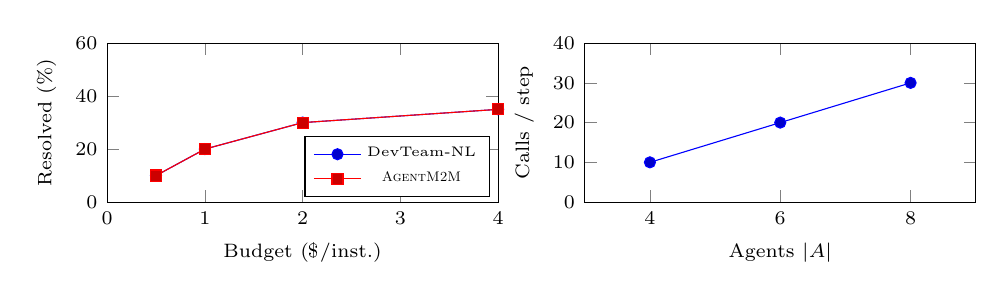
\begin{tikzpicture}
\begin{groupplot}[group style={group size=2 by 1, horizontal sep=1.1cm},
  width=0.54\columnwidth, height=3.6cm,
  label style={font=\scriptsize}, tick label style={font=\scriptsize}]
\nextgroupplot[xlabel={Budget (\$/inst.)}, ylabel={Resolved (\%)},
  xmin=0, xmax=4, ymin=0, ymax=60,
  legend style={font=\tiny, at={(0.98,0.03)}, anchor=south east}]
% PLACEHOLDER DATA
\addplot coordinates {(0.5,10) (1,20) (2,30) (4,35)};
\addplot coordinates {(0.5,10) (1,20) (2,30) (4,35)};
\legend{DevTeam-NL, \tool{}}
\phwatermark
\nextgroupplot[xlabel={Agents $|A|$}, ylabel={Calls / step},
  xmin=3, xmax=9, ymin=0, ymax=40, xtick={4,6,8}]
% PLACEHOLDER DATA
\addplot coordinates {(4,10) (6,20) (8,30)};
\phwatermark
\end{groupplot}
\end{tikzpicture}
\caption{RQ6: Resolve rate vs.\ budget on Verified (left); restorer and oracle
calls per agent step vs.\ team size (right).}
\label{fig:cost}
\end{figure}

%=============================================================
\subsection{Discussion}\label{subsec:discussion}
%=============================================================

\subsubsection{Where effects come from}
The chain \textsc{DevTeam-NL} $\to$ \textsc{Typed} $\to$ \tool{}, run with
identical agents, isolates typed outputs from correspondence-based
propagation. \hyp{If H1 holds while \textsc{Typed} is close to
\textsc{NL}, the effect is due to propagation, not to structured output.} The
forward-only ablation (H5) tests the specific mechanism of step \step{4}, and
H2 tests the prediction that cross-artifact mechanisms matter more for
multi-file changes.

\subsubsection{Consistency is not correctness}
If $\mathit{RA}$ lifts a wrong requirement from an underspecified issue,
\tool{} faithfully propagates it and converges on a consistent but wrong patch.
We therefore expect no gain on the instances that Lite-S
excludes~\cite{xia2025agentless}; \hyp{Table~\ref{tab:main} [confirms /
refutes] this}. This mirrors the unaddressed modes in Table~\ref{tab:mast}
(FM-1.1, 2.2, 2.6).

\subsubsection{Oracles are the weak link}
Corollary~\ref{cor:sound} is exact, but Proposition~\ref{prop:sem} is only as
good as $\epsilon_e$, and retries amplify oracle error. H7 and the bound check
of RQ5 quantify this; the actionable consequence is to replace judges with
executable checks wherever a relation admits one. A theory of bx with
stochastic restorers and fallible oracles, including their composition in
networks~\cite{stevens2020networks,klare2023termination}, is open.

\subsubsection{Adaptation and its limits}
Adaptation helps only when the initial team is wrong for the task; rollbacks,
$\theta$, and $A_{\max}$ act as hysteresis against oscillation. HOT synthesis
works when views share concepts; roles whose views share none require
hand-written templates, which is the engineering cost of \RC{3}.

\subsubsection{Cost of adoption}
Authoring \devteam{} took \fixme{N} person-hours and \fixme{N} lines of rules;
\textsc{MAGIS-M2M} took \fixme{N}. Because unconstrained edges degrade to
message passing, teams can adopt \tool{} incrementally.

\subsubsection{Threats to Validity}

\paragraph{Internal validity}
Unequal engineering effort could favor \tool{}; we use official baseline
implementations with the same back-end and budget, controlled variants that
share every prompt and tool, and a team design (\textsc{MAGIS-M2M}) whose roles
we did not choose. The frozen, development-only configuration guards against
tuning on test data. LLM non-determinism is handled by three runs and mixed
models.

\paragraph{External validity}
We study issue resolution, mostly in Python; other tasks and team structures
may benefit differently. Live and Pro broaden the repository base, but results
may not transfer to industrial settings.

\paragraph{Construct validity}
Resolve rates depend on benchmark tests; we therefore also report Lite-S.
MAST labels come from an LLM judge re-validated on our renderings. RQ2 metrics
rely on manual annotation with reported agreement. S1, S2, and S4 are
synthetic.

\paragraph{Conclusion validity}
Hypotheses and analyses are pre-registered; we report effect sizes with
confidence intervals and correct for multiple comparisons.

%=============================================================
\subsection{Preliminary Validation of a Working Implementation}\label{subsec:protovalidation}
%=============================================================
\noindent\textbf{Scope.} This subsection is deliberately distinct from RQ1--RQ6 above: it reports what an
open-source, algorithm-faithful implementation of \tool{} (Algorithms~\ref{alg:run}--\ref{alg:adapt}, in
TypeScript, part of the replication package of Section~\ref{sec:data}) actually does when driven by real,
local, freely available models. It is \emph{not} the pre-registered comparison against SWE-agent, OpenHands, Agentless, and MAGIS,
which needs the shared cloud back-end, budget, and baseline re-implementations of
Section~\ref{subsec:setup} and remains exactly as specified there. No hypothesis in Table~\ref{tab:hyp} is
tested here; H1--H7 remain open. Every number below is real -- no simulated, mocked, or hand-edited value.

\subsubsection{Implementation fidelity}
Every algorithm box in Section~\ref{sec:approach} has an independently unit-tested implementation (52
automated tests): $R_e^{\str}$ evaluation and $\mathit{Rule}_e$'s skeleton-with-holes construction;
\textsc{Lift}'s repair loop and stable-id \textsc{Instantiate}; \textsc{GuardedRestore}'s hippocratic
short-circuit (line~\ref{ln:rest-hip}) and hole-filling loop; \textsc{Propagate}'s fixed-order worklist and
per-edge budget $\ell$ -- including a hand-constructed three-edge cycle that exhausts $\ell$ and escalates
exactly as Proposition~\ref{prop:term} predicts; and \textsc{Adapt}'s transactional \textsc{Try}/rollback
under $\omega_{\mathit{init}}$ for the insert-impact-analyst scenario of Section~\ref{subsec:adapt}. One
additional test runs the RA$\leftrightarrow$TS slice of \devteam{} end to end against a live local model
with no mocking anywhere in the path, as a free, API-key-free correctness check.

\subsubsection{Multi-model validation on the running example}
We ran that same RA$\leftrightarrow$TS slice (edge $e_4$, the Duration.parse bug of
Section~\ref{subsec:example}) -- a real \textsc{Lift}, a real \textsc{Propagate} call invoking
\textsc{GuardedRestore}, a real, separately-prompted \textsc{FillHoles} call, and a real executable oracle
that runs the LLM-authored assertion against the buggy parser -- against every locally installed Ollama
model capable of instruction following (14 of 16 installed models; excluded one embedding model and one
model routed to a paid cloud proxy), two trials each, budget 8 turns, temperature 0.1. Table~\ref{tab:localmodels}
reports the results; raw data and per-trial logs are in the artifact's \code{evaluation/local-model-sweep/}.

\begin{table}[t]
\centering
\caption{Real, small-scale multi-model validation of \tool{}'s core loop (RA$\leftrightarrow$TS, $e_4$) on
Duration.parse, against locally-run Ollama models (2 trials each). Cost is agent turns to acceptance;
latency is per-trial wall-clock time. This is a validation that the mechanism works across models, not a
model-quality comparison -- the task is deliberately simple.}
\label{tab:localmodels}
\footnotesize
\begin{tabular}{@{}l r r r@{}}
\toprule
Model (params) & Success & Cost (turns) & Latency \\
\midrule
qwen2.5 (3B)             & 2/2 & 1 & 2.3s \\
llama3.1 (8B)            & 2/2 & 1 & 5.2s \\
qwen2.5-coder (7B)       & 2/2 & 1 & 4.0s \\
phi4-mini                & 2/2 & 1 & 3.7s \\
phi4 (14B)               & 2/2 & 1 & 4.8s \\
deepseek-r1 (14B)        & 2/2 & 1 & 6.8s \\
gemma4 (e4b)             & 2/2 & 1 & 10.7s \\
devstral (24B)           & 2/2 & 1 & 9.5s \\
mistral-small (24B)      & 2/2 & 1 & 12.6s \\
qwen3-coder (30B)        & 2/2 & 1 & 5.2s \\
llama3.3 (70B, q3\_K\_S) & 2/2 & 1 & 20.8s \\
\midrule
qwen3 (27B, variant A)   & 0/2 & -- & -- \\
qwen3 (27B, variant B)   & 0/2 & -- & -- \\
gpt-oss (20B)            & 0/2 & -- & -- \\
\bottomrule
\end{tabular}
\end{table}

11 of 14 models solved the scenario on both trials, each in a single \textsc{RunTeam} iteration (the same
iteration that lifts $r_1$ already triggers the \textsc{Propagate} call whose \textsc{GuardedRestore} on
$e_4$ both creates and accepts a correct repro test, matching step~\step{2} of
Section~\ref{subsec:example}), with latency scaling roughly with parameter count and quantization (2.3\,s
at 3B to 20.8\,s at 70B-q3).

\finding{The three failures were diagnosed, not merely observed. Probing the failing models directly with
the exact same prompt showed one \textsc{qwen3} variant returning an \emph{empty} response -- its hybrid
"thinking" mode had evidently consumed the entire bounded output budget on internal reasoning tokens before
an answer -- and \textsc{gpt-oss} returning unterminated chain-of-thought prose that never resolved to the
requested JSON. Both are reasoning-tuned models driven through Ollama's raw completion endpoint rather
than a chat-templated request; \textsc{deepseek-r1}, also reasoning-distilled, succeeded, so the failure is
architecture-specific rather than a property of reasoning models in general. In both failing cases
\textsc{Lift}'s repair loop behaved exactly as Algorithm~\ref{alg:lift} specifies: it re-prompted with the
explained validation errors up to $k_L$ times, received the same non-conforming output every time, and
\textsc{RunTeam} correctly reported budget-exhausted rather than a false accept. This is a model-router
integration gap (no chat-template-aware request path for reasoning-tuned models), not a defect in
\textsc{Lift} or \textsc{Propagate}.}

\subsubsection{Benchmark harness validation}
Independently, the SWE-bench-family fetchers of Section~\ref{subsec:setup} were exercised for real:
300/300 SWE-bench Lite~\cite{jimenez2024swebench}, 500/500 Verified~\cite{openai2024verified}, 1{,}000
Live~\cite{zhang2025swebenchlive}, and 642 Pro~\cite{deng2025swebenchpro} instances were fetched with every
required field populated (Lite-S's exact exclusion list~\cite{xia2025agentless} was not sourced this pass;
the filter mechanism is implemented, but its exclusion set is currently empty, so Lite-S coincides with
Lite here). The Docker execution harness that will run candidate patches for RQ1 was validated on three
real instances (\code{psf/requests-1963}, \code{psf/requests-2148}, \code{pallets/flask-4045}, re-verified
with a fresh, uncached run): applying each instance's gold patch resolved 3/3, and applying no patch
resolved 0/3 -- confirming the harness scores correctly before it is trusted to score any agent's output.
Live's and Pro's own Docker execution needs a harness adapter this pass does not implement (both use
image/test mechanics incompatible with the \texttt{swebench} package's execution path used here) and is
left for the RQ1 run proper. No baseline agent (SWE-agent, OpenHands, Agentless, MAGIS) was run in this
pass; doing so needs the shared cloud back-end and budget of the pre-registered protocol above, not a
change to the harness.



\section{Related Work}\label{sec:related}

\noindent\textbf{LLM multi-agent systems for SE.} He et al.\ survey LLM-based
multi-agent systems for SE~\cite{he2025lma}. MetaGPT~\cite{hong2024metagpt},
ChatDev~\cite{qian2024chatdev}, and MAGIS~\cite{tao2024magis} fix roles and
workflows; AutoGen~\cite{wu2024autogen} and CAMEL~\cite{li2023camel} program
conversations. Single-agent scaffolds~\cite{yang2024sweagent,wang2025openhands}
and pipelines~\cite{xia2025agentless} are strong baselines for issue
resolution. MAST~\cite{cemri2025mast} explains why teams fail; \tool{} turns
part of that diagnosis into checkable obligations.

\noindent\textbf{Structured coordination.} MetaGPT exchanges structured
documents~\cite{hong2024metagpt}; PatchBoard validates JSON-patch mutations of
one shared, task-specific state~\cite{zhang2026patchboard}; MCP and A2A
standardize transport~\cite{mcp2024,a2a2025}. \tool{} differs by keeping
\emph{heterogeneous} views and relating them by explicit, bidirectional
correspondences.

\noindent\textbf{Automated agent-system design.} GPTSwarm, ADAS, and AFlow
optimize agent graphs or programs~\cite{zhuge2024gptswarm,hu2025adas,zhang2025aflow},
largely offline; \tool{} adapts a running team and regenerates its
transformations with guarantees (Proposition~\ref{prop:adapt}).

\noindent\textbf{Consistency in MDE.} View-based development and consistency
preservation are well
studied~\cite{klare2021vitruvius,bruneliere2019views}, as are bx
semantics~\cite{stevens2010qvt,czarnecki2009bx,foster2007lenses,schurr1994tgg},
transformation networks~\cite{stevens2020networks,klare2023termination}, HOTs~\cite{tisi2009hot},
runtime models~\cite{blair2009runtime}, co-evolution~\cite{hebig2017coevolution},
and uncertainty~\cite{famelis2012partial,eramo2015uncertainty}. These works
assume deterministic, correct restorers and design-time evolution; \tool{}
contributes the treatment of stochastic restorers with oracle-checked
semantics and of runtime team evolution.



\section{Data Availability}\label{sec:data}
The anonymized replication package \fixme{URL} contains the implementation,
team definitions, pre-registration, prompts, per-run and per-instance
outcomes, annotation data, and analysis scripts. Table~\ref{tab:artifact} maps
the paper to the artifact.

\begin{table}[t]
\centering
\caption{Paper-to-artifact map \fixme{verify paths before submission}.}
\label{tab:artifact}
\scriptsize
\setlength{\tabcolsep}{3pt}
\begin{tabular}{@{}p{0.42\columnwidth} p{0.53\columnwidth}@{}}
\toprule
Paper element & Artifact location \\
\midrule
Defs.~\ref{def:mm}--\ref{def:model}, view metamodels & \code{teams/*/metamodels/*.ecore} \\
Def.~\ref{def:team}, team metamodel      & \code{agentm2m/team.ecore} \\
Alg.~\ref{alg:run} \textsc{RunTeam}      & \code{agentm2m/run.py} \\
Alg.~\ref{alg:lift} \textsc{Lift}        & \code{agentm2m/lift.py} \\
Alg.~\ref{alg:restore} \textsc{GuardedRestore} & \code{agentm2m/restore.py} \\
Alg.~\ref{alg:prop} \textsc{Propagate}   & \code{agentm2m/propagate.py} \\
Alg.~\ref{alg:adapt}, Def.~\ref{def:H}   & \code{agentm2m/adapt.py}, \code{hot.py} \\
Table~\ref{tab:corr}, $\Lambda$          & \code{teams/devteam/rules.py}, \code{adapt.yaml} \\
Table~\ref{tab:mast} mapping             & \code{docs/mast\_mapping.md} \\
Table~\ref{tab:hyp}, analyses            & \code{prereg/}, \code{analysis/} \\
Per-run outcomes, traces                 & \code{results/}, \code{traces/} \\
\bottomrule
\end{tabular}
\end{table}

\noindent The preliminary validation of Section~\ref{subsec:protovalidation} was run against a TypeScript
implementation with a different module layout than Table~\ref{tab:artifact}'s target structure above
(algorithms in \code{apps/engine/src/algorithms/*.ts}; benchmark fetchers and Docker harness in
\code{apps/bench/}; the multi-model sweep and its diagnosis in \code{evaluation/local-model-sweep/}) --
included in the same replication package, but not yet reorganized to match the paths above.

%=====================================================
%=====================================================
%=====================================================
%-------------------------[Conclusion]----------------
%=====================================================
%=====================================================
%=====================================================

\section{Conclusion}
\label{sec:conclusion}
\tool{} treats the collaboration of LLM agents as consistency management
among heterogeneous view models: typed hand-offs, explicit bidirectional
correspondences checked by rules and oracles, and a runtime team model whose
transformations are regenerated when the team adapts. We gave guarantees that
are exact for structure and probabilistic for semantics, and an evaluation
design that isolates each mechanism. \hyp{[Summarize the hypothesis outcomes.]}
Future work includes a theory of bx with stochastic restorers, learned
adaptation rules, and teams beyond issue resolution.

\section{Acknowledgments}
\fixme{Update this statement to name the AI tools actually used and their role
in preparing this manuscript, following the ICSE policy on generative AI.}


\clearpage
\bibliographystyle{IEEEtran}
\bibliography{agentm2m}

\end{document}
